\documentclass[xcolor=dvipsnames, compress, 10pt]{beamer}
\mode<presentation> {
	\usefonttheme{default}
	\usetheme{Ilmenau}
	\usecolortheme{default}
	%  	\usecolortheme{beaver}


	\defbeamertemplate*{headline}{miniframes theme no subsection}
	{%
		\begin{beamercolorbox}[colsep=1.5pt]{upper separation line head}
		\end{beamercolorbox}
		\begin{beamercolorbox}{section in head/foot}
			\vskip2pt\insertnavigation{\paperwidth}\vskip2pt
		\end{beamercolorbox}%
		\begin{beamercolorbox}[colsep=1.5pt]{lower separation line head}
		\end{beamercolorbox}
	}


	\defbeamertemplate*{footline}{myminiframes theme}
	{%
		\begin{beamercolorbox}[colsep=1.5pt]{upper separation line foot}
		\end{beamercolorbox}
		\begin{beamercolorbox}[ht=2.5ex,dp=1.125ex,%
			leftskip=.3cm,rightskip=.3cm plus1fil]{}%
			%{\usebeamerfont{title in head/foot}\insertshorttitle\hfill \insertshortinstitute}
			{\usebeamerfont{title in head/foot}\hfill \insertframenumber/\inserttotalframenumber}
		\end{beamercolorbox}%
		\begin{beamercolorbox}[colsep=1.5pt]{lower separation line foot}
		\end{beamercolorbox}
	}

	\setbeamertemplate{itemize items}[circle]
	\setbeamertemplate{enumerate items}[default]
	\setbeamerfont{caption}{size=\scriptsize}
	\setbeamertemplate{section in toc}[sections numbered]
	\setbeamertemplate{subsection in toc}[subsections numbered]
	\setbeamertemplate{caption}[numbered]
	\setbeamertemplate{footline}[miniframes theme no subsection]

	% \setbeamertemplate{bibliography entry title}{}
	% \setbeamertemplate{bibliography entry location}{}
	% \setbeamertemplate{bibliography entry note}{}
	% \setbeamercolor{bibliography entry author}{fg=black}
	% \setbeamercolor{bibliography entry location}{fg=black}
	% \setbeamercolor{bibliography entry note}{fg=black}
}


\usepackage{graphicx,epsf,subfigure}
\usepackage{amsmath,amsfonts,amsthm,amssymb,verbatim,booktabs,longtable,multirow,lscape}
\usepackage{enumerate, color, url}
\usepackage{dsfont}
\usepackage{setspace}
\usepackage{algorithm}
\usepackage{kotex}
\usepackage{adjustbox}
\usepackage{afterpage}
%\usepackage{enumitem}
\usepackage{bookmark}
\usepackage{hyperref}
\hypersetup{colorlinks=false, urlcolor=blue}
\usepackage{bm}
\usepackage{multirow}
\usepackage{geometry}
\usepackage{epsfig}
\usepackage{rotating}
\usepackage{tabularx}
\usepackage{array}
\usepackage{setspace} % \begin{spacing}

\theoremstyle{remark}
\newtheorem{remark}{Remark}[section]

\usepackage{mathtools}
\usepackage{makecell}

\usepackage{natbib}
\usepackage{tikz}
\usepackage{graphicx}
\graphicspath{{./}, {../figures/}}


% \newcommand{\bb}{\bm{b}}
% \newcommand{\bc}{\bm{c}}
% \newcommand{\bC}{\bm{C}}
% \newcommand{\bD}{\bm{D}}
% \newcommand{\bt}{\bm{t}}
% \newcommand{\bw}{\bm{w}}
% \newcommand{\bv}{\bm{v}}
% \newcommand{\bu}{\bm{u}}
% \newcommand{\bX}{\bm{X}}
% \newcommand{\bM}{\bm{M}}
% \newcommand{\bZ}{\bm{Z}}
% \newcommand{\hH}{\hat{H}}
% \newcommand{\bmu}{\bm{\mu}}
% \newcommand{\bxi}{\bm{\xi}}
% \newcommand{\bbeta}{\bm{\beta}}
% \newcommand{\blambda}{\bm{\lambda}}
% \newcommand{\btheta}{\bm{\theta}}
% \newcommand{\bgamma}{\bm{\gamma}}
% \newcommand{\bpi}{\bm{\pi}}
% \newcommand{\bphi}{\bm{\phi}}
% \newcommand{\bPhi}{\bm{\Phi}}
% \newcommand{\bpsi}{\bm{\psi}}
% \newcommand{\bthetah}{\hat{\bm{\theta}}}
% \newcommand{\bSigma}{\bm{\Sigma}}
% \newcommand{\bSigmah}{\widehat{\bm{\Sigma}}}
% \newcommand{\bOmega}{\bm{\Omega}}
% \newcommand{\CPO}{\text{CPO}}
% \newcommand{\LPML}{\text{LPML}}
% \newcommand{\as}{\text{ as }}
% \newcommand{\var}{\mbox{Var}}
% \newcommand{\cov}{\mbox{Cov}}
% \newcommand{\diag}{\mbox{Diag}}
% \newcommand{\gtheta}{g(\bm{\theta})}
% \newcommand{\gthetah}{g(\hat{\bm{\theta}})}

\newcommand{\ind}{d^{(in)}}
\newcommand{\outd}{d^{(out)}}
\newcommand{\dout}{d^{(in)}}
\newcommand{\din}{d^{(out)}}
\newcommand{\pout}{p^{(out)}}
\newcommand{\pin}{p^{(in)}}
\newcommand{\qout}{q^{(out)}}
\newcommand{\qind}{q^{(in)}}
\newcommand{\tq}{\tilde{q}}
\newcommand{\deltain}{\delta^{(in)}}
\newcommand{\deltaout}{\delta^{(out)}}

% \newcommand{\sigbeta}{\sigma_{\beta}}
% \newcommand{\siglamb}{\sigma_{\lambda_0}}
\def\code#1{\texttt{#1}}


\allowdisplaybreaks[0]


\title{Generating Networks with Predetermined Assortativity Measures}

\author{Yelie Yuan}
\institute{Department of Statistics, University of Connecticut}
\date{\today}


\begin{document}
\frame{\titlepage}

\begin{frame}{Abstract}

Assortativity coefficients are important metrics to analyze both directed and
undirected networks. In general, it is not guaranteed that the fitted network
will always agree with the assortativity coefficients in the given network and
the structure of directed networks is more complicated than the undirected ones.
Therefore, we provide a remedy by proposing a degree-preserving rewiring
algorithm, called DiDPR, for rewiring directed networks toward given directed
assortativity coefficients. We construct the joint degree distribution of the
target network by accounting for the four directed assortativity coefficients
simultaneously, provided that they are attainable, and obtain the desired joint
distribution by solving a convex optimization problem. Our algorithm also helps
check the attainability of the given assortativity coefficients.
	
\end{frame}


\begin{frame}
	\frametitle{Overview}
	\tableofcontents
\end{frame}

%------------------------------------------------

\section{Background}

\begin{frame}{What is a network?}

A network (or graph) $G(V, E)$ is an object composed of vertices (or nodes)
connected by edges; $V$ represents the node set and $E$
represents the edge set.


The structure of a network can be represented by a matrix. 
For a directed network (bottom),
the adjacency matrix may not symmetric.

\vspace{0.5cm}

\begin{columns}
	\begin{column}{0.5\textwidth}
		\centering
		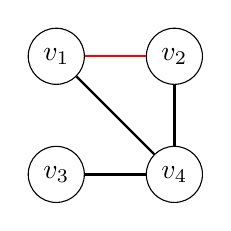
\begin{tikzpicture}
    \draw (0, 0) node[draw = black, circle] (v1) {$v_1$};
    \draw (1.5, 0) node[draw = black, circle] (v2) {$v_2$};
    \draw (0, -1.5) node[draw = black, circle] (v3) {$v_3$};
    \draw (1.5, -1.5) node[draw = black, circle] (v4) {$v_4$};
    \draw[thick, red] (v1) -- (v2);
    \draw[thick] (v1) -- (v4);
    \draw[thick] (v2) -- (v4);
    \draw[thick] (v3) -- (v4);
\end{tikzpicture}
	\end{column}
	\begin{column}{0.5\textwidth}
		\centering
		\begin{align*}
			A_1 = 
			\begin{pmatrix*}
			0 & \color{red} 1 & 0 & 1 \\
			\color{red} 1 & 0 & 0 & 1 \\
			0 & 0 & 0 & 1 \\
			1 & 1 & 1 & 0
			\end{pmatrix*}
		\end{align*}
	\end{column}
\end{columns}

\vfill

\begin{columns}
	\begin{column}{0.5\textwidth}
		\centering
		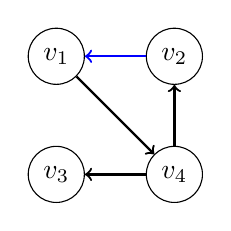
\begin{tikzpicture}
    \draw (0, 0) node[draw = black, circle]
    (v1) {$v_1$};
    \draw (1.5, 0) node[draw = black, circle]
    (v2) {$v_2$};
    \draw (0, -1.5) node[draw = black, circle] (v3) {$v_3$};
    \draw (1.5, -1.5) node[draw = black, circle] (v4) {$v_4$};
    \draw[->, thick] (v1) -- (v4);
    \draw[->, thick, blue] (v2) -- (v1);
    \draw[->, thick] (v4) -- (v2);
    \draw[->, thick] (v4) -- (v3);
\end{tikzpicture}
	\end{column}
	\begin{column}{0.5\textwidth}
		\centering
		\begin{align*}
			A_2 = 
			\begin{pmatrix*}
				0 & 0 & 0 & 1 \\
				\color{blue}{1} & 0 & 0 & 0 \\
				0 & 0 & 0 & 0 \\
				0 & 1 & 1 & 0
			\end{pmatrix*}
		\end{align*}
	\end{column}
\end{columns}
	
\end{frame}

%------------------------------------------------

\begin{frame}{Node degree}

\begin{columns}
	\begin{column}{0.75\textwidth}
		Undirected networks
		\begin{itemize}
			\item Degree of a node is the number of edges connected to
			it; $d_{v_1} = d_{v_2} = 2$, $d_{v_3} = 1$, $d_{v_4} = 3$.
		\end{itemize}
	\end{column}
	\begin{column}{0.2\textwidth}
		\scalebox{0.7}{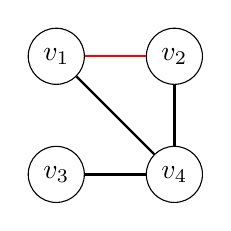
\begin{tikzpicture}
    \draw (0, 0) node[draw = black, circle] (v1) {$v_1$};
    \draw (1.5, 0) node[draw = black, circle] (v2) {$v_2$};
    \draw (0, -1.5) node[draw = black, circle] (v3) {$v_3$};
    \draw (1.5, -1.5) node[draw = black, circle] (v4) {$v_4$};
    \draw[thick, red] (v1) -- (v2);
    \draw[thick] (v1) -- (v4);
    \draw[thick] (v2) -- (v4);
    \draw[thick] (v3) -- (v4);
\end{tikzpicture}}
	\end{column}
\end{columns}

\vspace{0.2cm}

\begin{columns}
	\begin{column}{0.75\textwidth}
		Directed networks
		\begin{itemize}
			\item Out-degree of a node is the number of edges it sends;
			$\outd_{v_1} = \outd_{v_2} = 1$, $\outd_{v_3} = 0$, 
			$\outd_{v_4} = 2$.
			\item In-degree of a node is the number of edges it receives;
			$\ind_{v_1} = \ind_{v_2} = \ind_{v_3} = \ind_{v_4} = 1$.
			\item For edge $\color{blue}{(v_2, v_1)}$, $v_2$ is the source node,
			$v_1$ is the target node.
		\end{itemize}
	\end{column}
	\begin{column}{0.2\textwidth}
		\scalebox{0.7}{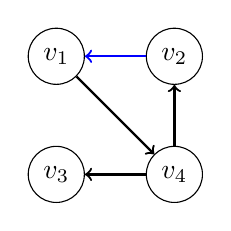
\begin{tikzpicture}
    \draw (0, 0) node[draw = black, circle]
    (v1) {$v_1$};
    \draw (1.5, 0) node[draw = black, circle]
    (v2) {$v_2$};
    \draw (0, -1.5) node[draw = black, circle] (v3) {$v_3$};
    \draw (1.5, -1.5) node[draw = black, circle] (v4) {$v_4$};
    \draw[->, thick] (v1) -- (v4);
    \draw[->, thick, blue] (v2) -- (v1);
    \draw[->, thick] (v4) -- (v2);
    \draw[->, thick] (v4) -- (v3);
\end{tikzpicture}}
	\end{column}
\end{columns}

\vfill

In the following discussion, we focus on directed networks.

\end{frame}

%------------------------------------------------

\begin{frame}{Distributions}

$e_{k\ell}^{(a, b)}$: the probability that a randomly chosen edge connects
to a source node of type $a$ degree $k$ and a target node of type $b$
degree $\ell$ for $a, b \in \{out, in\}$.

% $p_k^{(a)}$: the probability that a randomly chosen node has type $a$
% degree $k$.

$q_k^{(a)}$: the probability that a randomly chosen edge starts from a
source node of type $a$ degree $k$.

$\tilde q_k^{(a)}$: the probability that a randomly chosen edge points to
a target node of type $a$ degree $k$.

\vspace{0.2cm}

By definition, we have 
\begin{align*}
	% q_k^{a} & = \frac{k \, p_k^{a}}{\sum_j j \, p_j^{a}}, \qquad
	% q_k^a = \sum_j e_{jk}^a,\\
	% e_{jk}^a &= e_{kj}^a, \qquad \sum_{j\,k} e_{jk}^a = 1.\\
	q_k^{(a)} = \sum_\ell e_{k\ell}^{(a, b)}, \qquad 
	\tilde q_\ell^{(b)} = \sum_k e_{k\ell}^{(a, b)}, \qquad
	\sum_{k \ell} e_{k\ell}^{(a, b)} = 1.
\end{align*}

\end{frame}
	
%------------------------------------------------


\begin{frame}{Assortativity}

Assortativity is a metric measuring the tendency that nodes in a network are
connected to others with similar characteristics, for example,
node degrees.

\vspace{0.1cm}

Four types of directed assortativity measures:
\begin{equation*}
	% \label{eq:4dassort}
  	r(a, b) = 
    \frac{\sum_{k,\ell} k\ell \left(e^{(a,b)}_{k\ell} - q_k^{(a)} 
    \tq_\ell^{(b)}\right)}{\sigma_q^{(a)} \sigma_{\tq}^{(b)}},
    \qquad a,b \in \{out,in\},
\end{equation*} 
where 
\[
\sigma_q^{(a)} = 
\sqrt{\sum_k k^2 q_k^{(a)} - \left(\sum_k k q_k^{(a)}\right)^2}, 
\sigma_{\tq}^{(b)} = 
\sqrt{\sum_\ell \ell^2 \tq_l^{(b)} - 
	\left(\sum_\ell \ell \tq_\ell^{(a)}\right)^2}
\]
are standard deviations of $q_k^{(a)}$ and $\tq_l^{(b)}$, 
respectively.

% \vspace{0.1cm}


% In assortative networks, high-degree nodes, 
% or nodes with many edges, tend to connect to other high-degree nodes.
% In disassortative networks, high-degree nodes tend to 
% connect to low-degree nodes.

% \begin{columns}
% 	\begin{column}{0.5\textwidth}
% 		\centering
% 		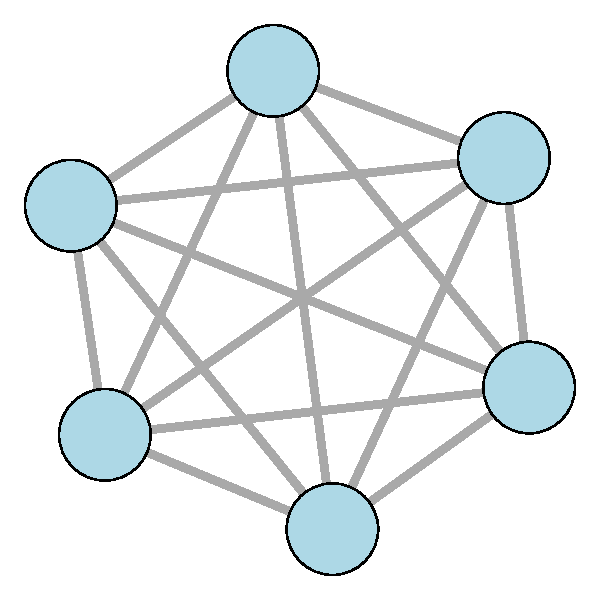
\includegraphics[width=0.3\linewidth]{full_graph.pdf}\\
% 		Assortative
% 	\end{column}
% 	\begin{column}{0.5\textwidth}
% 		\centering
% 		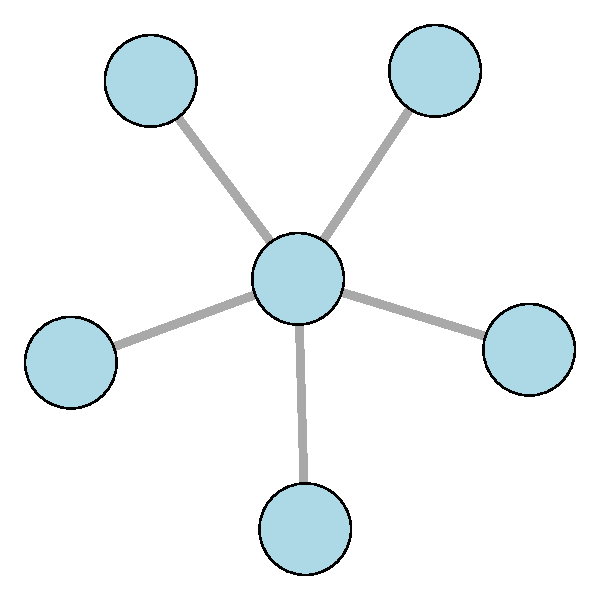
\includegraphics[width=0.3\linewidth]{star_graph.pdf}\\
% 		Disassortative
% 	\end{column}
% \end{columns}

\end{frame}


%------------------------------------------------

\begin{frame}{Main task}


Given an initial directed network and four target assortativity coefficients,
how should we modify the network to obtain the 
target assortativity levels while keeping the out- and in-degree distributions
unchanged?
	
	
\end{frame}


%------------------------------------------------

\begin{frame}{Degree-preserving rewiring (DPR)}

The rationale of DPR is that the degree sequence is unaffected, whilst the
assortativity coefficients change. 

\vspace{0.1cm}

The distributions $q_{k}^{(a)}$ and 
$\tilde q_{k}^{(a)}$are unchanged, but the joint degree distributions
$e_{k\ell}^{(a, b)}$ and assortativity 
coefficients $r(a, b)$ may be affected.

\vspace{0.1cm}

\begin{columns}
	\begin{column}{0.4\textwidth}
		\hfill
		\scalebox{0.6}{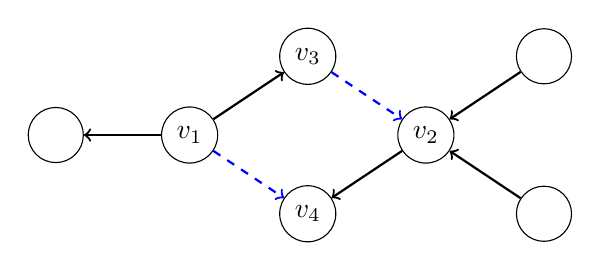
\begin{tikzpicture}
      \draw (-1.5, 0) node[draw = black, circle, minimum size = 0.7cm] (v1) {$v_1$};
      \draw (1.5, 0) node[draw = black, circle, minimum size = 0.7cm] (v2) {$v_2$};
      \draw (0, 1) node[draw = black, circle, minimum size = 0.7cm] (v3) {$v_3$};
      \draw (0, -1) node[draw = black, circle, minimum size = 0.7cm](v4) {$v_4$};
    %   \draw (-3, 1) node[draw = black, circle, minimum size = 0.7cm] (v5) {};
      \draw (-3.2, 0) node[draw = black, circle, minimum size = 0.7cm] (v6) {};
      \draw (3, 1) node[draw = black, circle, minimum size = 0.7cm] (v7) {};
      \draw (3, -1) node[draw = black, circle, minimum size = 0.7cm] (v8) {};
  
      \draw[->, thick, dashed, blue] (v1) -- (v4);
      \draw[->, thick, dashed, blue] (v3) -- (v2);
      \draw[->, thick] (v1) -- (v3);
    %   \draw[->, thick] (v5) -- (v1);
      \draw[->, thick] (v1) -- (v6);
      \draw[->, thick] (v2) -- (v4);
      \draw[->, thick] (v7) -- (v2);
      \draw[->, thick] (v8) -- (v2);
  \end{tikzpicture}}
	\end{column}
	\begin{column}{0.6\textwidth}
		\begin{align*}
			&r(out, out) = -0.42 \quad r(out, in) = -0.84\\
			&r(in, out) = -0.35 \quad r(in, in) = 0.07
		\end{align*}
	\end{column}
\end{columns}

\vspace{0.2cm}

\begin{columns}
	\begin{column}{0.4\textwidth}
		\hfill
		\scalebox{0.6}{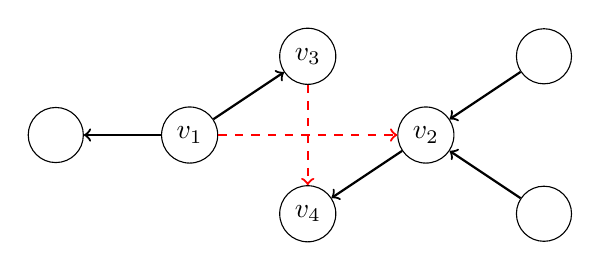
\begin{tikzpicture}
    \draw (-1.5, 0) node[draw = black, circle, minimum size = 0.7cm] (v1) {$v_1$};
    \draw (1.5, 0) node[draw = black, circle, minimum size = 0.7cm] (v2) {$v_2$};
    \draw (0, 1) node[draw = black, circle, minimum size = 0.7cm] (v3) {$v_3$};
    \draw (0, -1) node[draw = black, circle, minimum size = 0.7cm](v4) {$v_4$};
  %   \draw (-3, 1) node[draw = black, circle, minimum size = 0.7cm] (v5) {};
    \draw (-3.2, 0) node[draw = black, circle, minimum size = 0.7cm] (v6) {};
    \draw (3, 1) node[draw = black, circle, minimum size = 0.7cm] (v7) {};
    \draw (3, -1) node[draw = black, circle, minimum size = 0.7cm] (v8) {};

    \draw[->, thick, dashed, red] (v1) -- (v2);
    \draw[->, thick, dashed, red] (v3) -- (v4);
    \draw[->, thick] (v1) -- (v3);
  %   \draw[->, thick] (v5) -- (v1);
    \draw[->, thick] (v1) -- (v6);
    \draw[->, thick] (v2) -- (v4);
    \draw[->, thick] (v7) -- (v2);
    \draw[->, thick] (v8) -- (v2);
\end{tikzpicture}}
	\end{column}
	\begin{column}{0.6\textwidth}
		\begin{align*}
			&r(out, out) = 0.17 \quad r(out, in) = -0.50\\
			&r(in, out) = -0.63 \quad r(in, in) = -0.09
		\end{align*}
	\end{column}
\end{columns}


\end{frame}

%------------------------------------------------

\begin{frame}{Bridge the four $e_{k\ell}^{(a, b)}$}

\vspace{0.2cm}

Let $\nu_{k\ell}$ be the proportion of nodes with out-degree $k$ and in-degree
$\ell$. Define $\eta_{ijk\ell} \ge 0$ as the proportion of directed edges
linking a source node with out-degree~$i$ and in-degree $j$ to a target node
with out-degree $k$ and in-degree $\ell$. 

\vspace{0.2cm}

Then the following relations hold, which are the building blocks for the
development of our algorithm:
\begin{align*}
	\sum_{j, \ell} \eta_{ijk\ell} = e^{(out, out)}_{ik}, 
	&\qquad
	\sum_{j, k} \eta_{ijk\ell} = e^{(out, in)}_{i\ell}, 
	\qquad
	\sum_{k, \ell} \eta_{ijk\ell} = \frac{i \, \nu_{ij}}{\sum_{i, j} i 
	\,\nu_{ij}},\\
	\sum_{i, \ell} \eta_{ijk\ell} = e^{(in, out)}_{jk}, 
	&\qquad 
	\sum_{i, k} \eta_{ijk\ell} = e^{(in, in)}_{j\ell}, 
	\qquad
	\sum_{i, j} \eta_{ijk\ell} = 
	\frac{\ell \, \nu_{k\ell}}{\sum_{k, \ell} \ell\, \nu_{k\ell}}.
\end{align*}
	
\end{frame}

%------------------------------------------------

\begin{frame}{Bridge the four $e_{k\ell}^{(a, b)}$}

Recall the four types of directed assortativity measures:
\begin{align*}
	r(a, b) &= 
	\frac{\sum_{k,\ell} k\ell (e^{(a,b)}_{k\ell} - q_k^{(a)} \tq_\ell^{(b)})}{\sigma_q^{(a)} \sigma_{\tq}^{(b)}} \\
	&= \frac{1}{\sigma_q^{(a)} \sigma_{\tq}^{(b)}} 
		\left(\sum_{k,\ell} k\ell e^{(a,b)}_{k\ell}\right) - 
	\frac{1}{\sigma_q^{(a)} \sigma_{\tq}^{(b)}} 
		\left(\sum_{k,\ell} k\ell q_k^{(a)} \tq_\ell^{(b)}\right).
\end{align*}

% Additionally, we write $q$
% and $\tq$ as functions of $\eta_{ijk\ell}$ and $\nu_{k\ell}$:
% \begin{align*}
% 	\sum_{j, k, \ell} \eta_{ijk\ell} = \frac{\sum_j i \,
% 	\nu_{ij}}{\sum_{i, j} i \, \nu_{ij}} = \qout_i, 
% 		&\qquad 
% 		\sum_{i, k, \ell} \eta_{ijk\ell} = \frac{\sum_i i \,
% 		\nu_{ij}}{\sum_{i, j} i \, \nu_{ij}} = \qind_j,
% 		\\
% 		\sum_{i, j, l} \eta_{ijk\ell} = \frac{\sum_l l \,
% 		\nu_{k\ell}}{\sum_{k, \ell} l \, \nu_{k\ell}} = \tq_k^{(out)}, 
% 		&\qquad 
% 		\sum_{i, j, k} \eta_{ijk\ell} = \frac{\sum_k l \,
% 		\nu_{k\ell}}{\sum_{k, \ell} l \, \nu_{k\ell}} = \tq_l^{(in)}.
% \end{align*}

\vspace{0.1cm}

With the relations between $e_{k\ell}^{(a, b)}$ and $\eta_{ijk\ell}$, all
assortativity coefficients, $r(a,b)$, are linear functions of $\eta_{ijk\ell}$.
The quantities like $q_k^{(a)}$, $\tq_l^{(b)}$, $\sigma_q^{(a)}$ and
$\sigma_{\tq}^{(b)}$ are not affected by edge rewiring.

\vspace{0.1cm}

The problem boils down to the following:
\begin{itemize}
	\item How to find an $\eta_{ijk\ell}$ with a given 
	network and four target assortativity coefficients?
	\item How to rewire the given network toward the constructed 
	$\eta_{ijk\ell}$?
\end{itemize}


\end{frame}


%------------------------------------------------


\section{Directed network degree-preserving rewiring (DiDPR) algorithm}


\begin{frame}{Find an $\bm{\eta}$}

$r^*(a, b), a, b \in \{out, in\}$ are the predetermined values of 
the four directed assortativity measures;
$f(\cdot)$ is a convex function;
$\mathcal{D}^{(in)}$ and $\mathcal{D}^{(out)}$ are the support of
the empirical distribution of the in-degrees and out-degrees, respectively.


We set up the following convex optimization problem to solve for an
$\boldsymbol{\eta} := \{\eta_{ijk\ell}\}$: 
\begin{align*}
  \min_{\bm{\eta}} \quad &f(\bm{\eta}),                            
  \nonumber\\
  \textrm{s.t.}  \quad  &-\eta_{ijk\ell} \le 0,
  \quad \forall i,k \in \mathcal{D}^{(out)}, 
  \quad \forall j,\ell \in \mathcal{D}^{(in)}, 
  \\
  &\sum_{k, \ell} \eta_{ijk\ell} = \frac{i \nu_{ij}}{\sum_{i, j} i \nu_{ij}},
  \quad \forall i \in \mathcal{D}^{(out)}, 
  \quad \forall j \in \mathcal{D}^{(in)},
  \nonumber\\
  & \sum_{i, j} \eta_{ijk\ell} = \frac{\ell \nu_{k\ell}}{\sum_{k, \ell} \ell \nu_{k\ell}},
  \quad \forall k \in \mathcal{D}^{(out)}, 
  \quad \forall \ell \in \mathcal{D}^{(in)},                    
  \nonumber\\
  &r\left(a, b \right) = r^* \left(a, b \right),
  \quad  a, b \in \{out, in\}.
  \nonumber
\end{align*}

\end{frame}


%------------------------------------------------

\begin{frame}{Rewiring process}
	
% More specifically, given an initial network $G_0(V, E)$ and four 
% predetermined assortativity coefficients, we first solve the convex 
% optimization problem defined above to obtain $\bm{\eta}$.
% Then we proceed to the (degree-preserving) rewiring procedure. 
At each 
rewiring step, we randomly select a pair of edges
$(v_1, v_2), (v_3, v_4)$. Measure the out- and in-degrees 
$i_1 = \dout_{v_1}$, $j_1 = \din_{v_1}$, 
$k_1 = \dout_{v_2}$, $\ell_1 = \din_{v_2}$, 
$i_2 = \dout_{v_3}$, $j_2 = \din_{v_3}$, 
$k_2 = \dout_{v_4}$ and $\ell_2 = \din_{v_4}$.
We then replace the selected $(v_1, v_2)$ and $(v_3, v_4)$ with
$(v_1, v_4)$ and $(v_3, v_2)$ with probability
\begin{equation*}
   \rho = \begin{cases}
   	\left(\eta_{i_1 j_1 k_2 \ell_2}\, \eta_{i_2 j_2 k_1 \ell_1}\right)/
    \left(\eta_{i_1 j_1 k_1 \ell_1}\, \eta_{i_2 j_2 k_2 \ell_2}\right), 
    &\qquad \text{if }
    \frac{\eta_{i_1 j_1 k_2 \ell_2}\, \eta_{i_2 j_2 k_1 \ell_1}}
	{\eta_{i_1 j_1 k_1 \ell_1}\, \eta_{i_2 j_2 k_2 \ell_2}} < 1;
    \\ 1, &\qquad \text{otherwise}.
    \end{cases}
\end{equation*} 

\vspace{0.2cm}

Iteratively continue the rewiring steps for $T$ times, and obtain the resulting
network $G(V, E)$.

\end{frame}


%------------------------------------------------

\begin{frame}{Properties}

Out- and in-degree distributions are unchanged.

\vspace{0.2cm}

The algorithm is \emph{ergodic} over the 
collection of networks with given out- and in-degree sequences 
(denoted by $\mathcal{G}$), as any network in $\mathcal{G}$ can be 
reached within a finite number of rewiring steps. 

\vspace{0.2cm}

The algorithm satisfies the \emph{detailed balance} condition, 
i.e., for any 
two configurations $G_1, G_2 
\in \mathcal{G}$, it follows from the probability $\rho$ that 
\[
\Pr(G_1) \Pr(G_1 \to G_2) = \Pr(G_2) \Pr(G_2 \to G_1),
\]
where $\Pr(G_1)$ denotes the probability of sampling configuration 
$G_1 \in \mathcal{G}$, and $\Pr(G_1 \to G_2)$ is the transition 
probability from $G_1$ to $G_2$. 

\end{frame}


%------------------------------------------------

\begin{frame}{Assortativity coefficient bounds}

The four target assortativity coefficients, $r^*(a, b)$, 
$a, b \in \{out, in\}$, are naturally bounded
between $-1$ and $1$. 
However, based on the structure of $G_0(V, E)$, 
we cannot arbitrarily set four targets, $r^*(a, b)$, $a, b \in 
\{out, in\}$, to any values within the range of $[-1, 1]$ while 
preserving $\bm{\nu}$, since certain combinations of the target values 
may not be achievable. 

\vspace{0.2cm}

Recall that quantities like $q_k^{(a)}$, $\tq_l^{(b)}$, 
$\sigma_q^{(a)}$ and $\sigma_{\tq}^{(b)}$ 
remain unchanged throughout the rewiring process, and
$r(a, b)$ is a linear function of 
$\sum_{k, \ell} k\ell e^{\left(a, b\right)}_{k\ell}$,

\begin{align*}
	r(a, b) &= \frac{1}{\sigma_q^{(a)} \sigma_{\tq}^{(b)}} 
		\left(\sum_{k,\ell} k\ell e^{(a,b)}_{k\ell}\right) - 
	\frac{1}{\sigma_q^{(a)} \sigma_{\tq}^{(b)}} 
		\left(\sum_{k,\ell} k\ell q_k^{(a)} \tq_\ell^{(b)}\right).
\end{align*}

\end{frame}


%------------------------------------------------

\begin{frame}{Assortativity coefficient bounds}

Without loss of generality, we take 
$r^*(out, out)$ as an example. The lower bound of $r^*(out, out)$ is obtained
by solving the following convex optimization problem:
\begin{align*}
	\min_{\bm{\eta}} \qquad &
	f^{(out,out)}(\bm{\eta}) := \sum_{i, k}ik 
	\left(\sum_{j, \ell} \eta_{ijk\ell}\right),
	\\ \textrm{s.t.} \qquad & -\eta_{ijk\ell} \le 0, 
	\quad \forall i,k \in \mathcal{D}^{(out)}, 
	\quad \forall j,\ell \in \mathcal{D}^{(in)}, 
	\\ &\sum_{k, \ell} \eta_{ijk\ell} = 
	\frac{i \nu_{ij}}{\sum_{i, j} i \nu_{ij}},
	\quad \forall i \in \mathcal{D}^{(out)}, 
	\quad \forall j \in \mathcal{D}^{(in)},
	\\ &\sum_{i, j} \eta_{ijk\ell} = 
	\frac{\ell \nu_{k\ell}}{\sum_{k, \ell} \ell \nu_{k\ell}},
	\quad \forall k \in \mathcal{D}^{(out)}, 
	\quad \forall \ell \in \mathcal{D}^{(in)}.
\end{align*}
Analogously, we obtain the upper bound of $r^{*}(out, out)$ by 
solving the optimization problem with the objective function 
$-f^{(out, out)}(\bm{\eta})$, while keeping all of the
constraints unchanged.
	
	
\end{frame}

%------------------------------------------------

\section{Simulation and application}


\begin{frame}{Erd\"{o}s--R\'{e}nyi (ER) networks}


The Erd\"{o}s--R\'{e}nyi (ER) model~\citep{Erdos1959on, Gilbert1959random} is
governed by two parameters: the number of nodes $n$ and the probability of an
edge between two nodes $p \in [0, 1]$. 

\vspace{0.2cm}

We consider an extension of the traditional ER random network model allowing
edge direction and self-loops. In directed ER networks, all of the edges are
generated independently.
	
\end{frame}

%------------------------------------------------

\begin{frame}{Erd\"{o}s--R\'{e}nyi (ER) networks}

Fix $n = 1000$, and set $p \in \{0.05, 0.1, 0.2, 0.4\}$. The target 
assortativity
values are given by $r^*(out, out) = 0.6$, $r^*(out, in) = 0.5$, 
$r^*(in, out) = -0.4$ and $r^*(in, in) = -0.3$. 
For each combination of $n$ and $p$, we
generate $100$ independent networks. Each rewiring iteration contains
$10^4$ rewiring steps.
\begin{figure}[tbp]
	\centering
	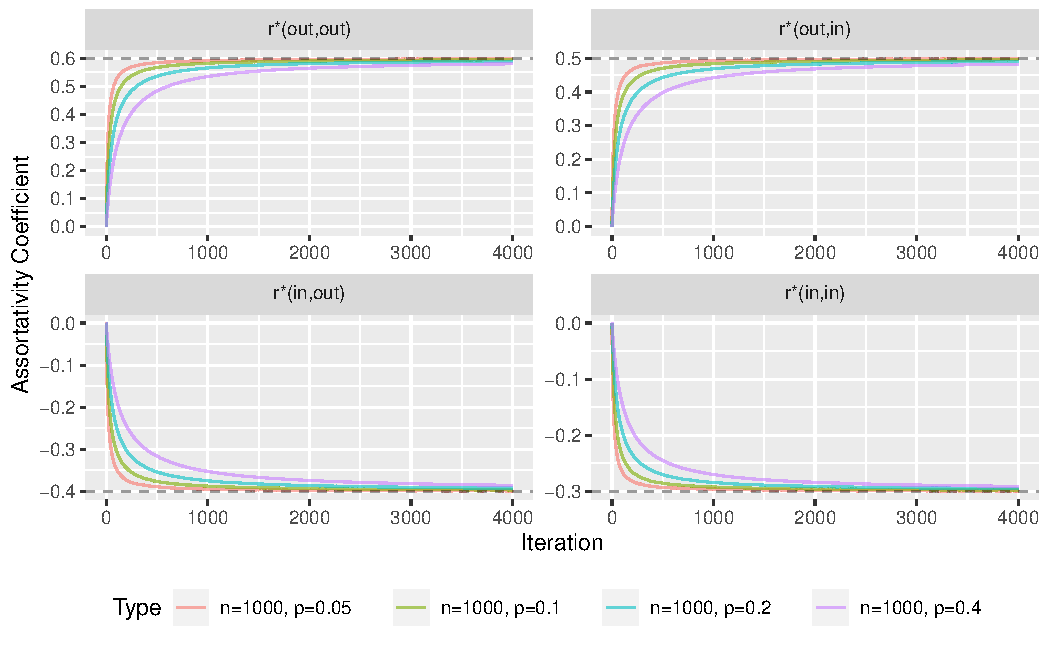
\includegraphics[width = 0.8\textwidth]{ER_fix_N1000_archive.pdf}
\end{figure}
	
\end{frame}

%------------------------------------------------

\begin{frame}{Preferential attachment (PA) networks}

The preferential attachment (PA) model is a generative probabilistic model such
that nodes with large degrees are more likely to attract newcomers than those
with small degrees~\citep[e.g.,][]{Barabasi1999emergence, Krapivsky2001degree,
Krapivsky2001organization}. It is a more realistic model for many real network
data than the ER model. We consider the directed PA (DPA) model given
in~\cite{Bollobas2003proceedings}, which has five parameters $(\alpha, \beta,
\gamma, \deltain, \deltaout)$ subject to $\alpha + \beta + \gamma = 1$.

\vspace{0.2cm}

We assume there are three edge-creation scenarios ($\alpha$, $\beta$ and
$\gamma$, from left to	right):
	
\begin{figure}
	\centering
	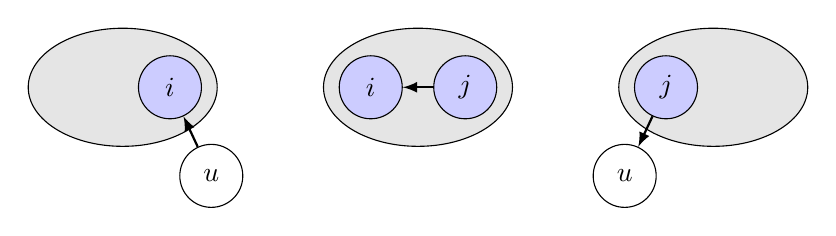
\begin{tikzpicture}[scale=0.75]
    \draw[fill = gray!20] (-5, 0) ellipse (1.6 and 1) ;
    \draw (-4.2, 0) node[draw = black, circle, minimum 
    size =
    0.8cm, fill = blue!20] (i1)	{$i$} ;
    \draw (-3.5, -1.5) node[draw = black, circle, 
    minimum 
    size = 0.8cm] (u1)	{$u$} ;
    \draw[-latex, thick] (u1) -- (i1) ;
    \draw[fill = gray!20] (0, 0) ellipse (1.6 and 1) ;
    \draw (-0.8, 0) node[draw = black, circle, minimum 
    size =
    0.8cm, fill = blue!20] (i2)	{$i$} ;
    \draw (0.8, 0) node[draw = black, circle, minimum 
    size = 0.8cm, fill = blue!20] (j1)	{$j$} ;
    \draw[-latex, thick] (j1) -- (i2) ;
    \draw[fill = gray!20] (5, 0) ellipse (1.6 and 1) ;
    \draw (4.2, 0) node[draw = black, circle, minimum 
    size =
    0.8cm, fill = blue!20] (j2)	{$j$} ;
    \draw (3.5, -1.5) node[draw = black, circle, minimum 
    size = 0.8cm] (u2)	{$u$} ;
    \draw[-latex, thick] (j2) -- (u2) ;
\end{tikzpicture}
\end{figure}

\end{frame}

%------------------------------------------------

\begin{frame}{Preferential attachment (PA) networks}

We fix $\deltaout = \deltain = 1$; consider $\beta \in \{0.1, 0.2, 0.3, 0.4\}$,
and set the corresponding $\alpha = \gamma$ such that 
$\alpha + \beta + \gamma = 1$.

% We do not allow $\beta$ to take large values in our simulations since
% otherwise the $\beta$-scenario will dominate the network evolution, decreasing
% the number of nodes created during the entire network growth. 


$100$ independent DPA networks are generated and the assortativity
coefficients are collected for every $10^3$ rewiring steps.

\begin{figure}
	\centering
	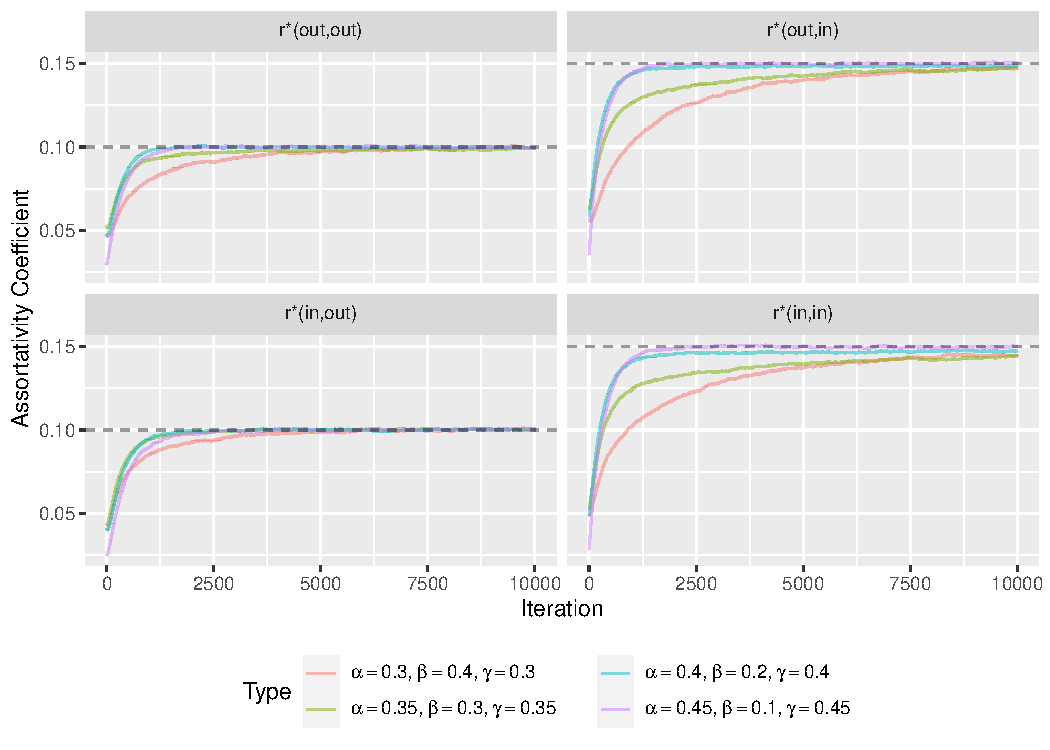
\includegraphics[width = 0.7\textwidth]{alpha_eq_gamma_beta1-4_archive.pdf}
\end{figure}

\end{frame}

%------------------------------------------------

\begin{frame}{Facebook wall post network}


Nodes in the Facebook wall post network correspond to
Facebook users, and each directed edge $(v_i,v_j)$ represents 
the event that user~$v_i$ writes a post on the wall of user~$v_j$.

\begin{itemize}
	\item Data source:
	\href{http://konect.cc/networks/facebook-wosn-wall/}{KONECT}~\citep{Kunegis2013konect};
	\item Period: 2007/07/01 to 2007/11/30;
	\item Node number: 16,549;
	\item Edge number: 147,063;
	\item Assortativity coefficients: $r(out, out) = 0.44$, 
	$r(out, in) = 0.49$, $r(in, out) = 0.46$, 
	and $r(in, in) = 0.41$;
	\item Fitted model: directed preferential 
	attachment (DPA) network~\citep{Bollobas2003proceedings};
	\item Estimation method: extreme value method~\citep{Wan2020extreme}.
\end{itemize}

% We fit a DPA model to the selected network, and 
% estimate the parameters via an {\em extreme value} (EV) method. The 
% fitted model well captures the features of out- and in-degree 
% distributions of the network data, but fails to characterize the 
% assortativity structure accurately. By applying the DiDPR algorithm, 
% we see that four assortativity coefficients of the fitted model are 
% close to the counterparts of the selected network.

\end{frame}

%------------------------------------------------

\begin{frame}{Facebook wall post network}

We then generate $100$ independent DPA networks of size $147,063$ and overlay
the marginal out- and in-degree distributions of the simulated networks and
their empirical counterparts from the selected network.

% The fitted model well captures the features of out- and in-degree 
% distributions of the network data, but fails to characterize the 
% assortativity structure accurately.

\begin{figure}
	\centering
	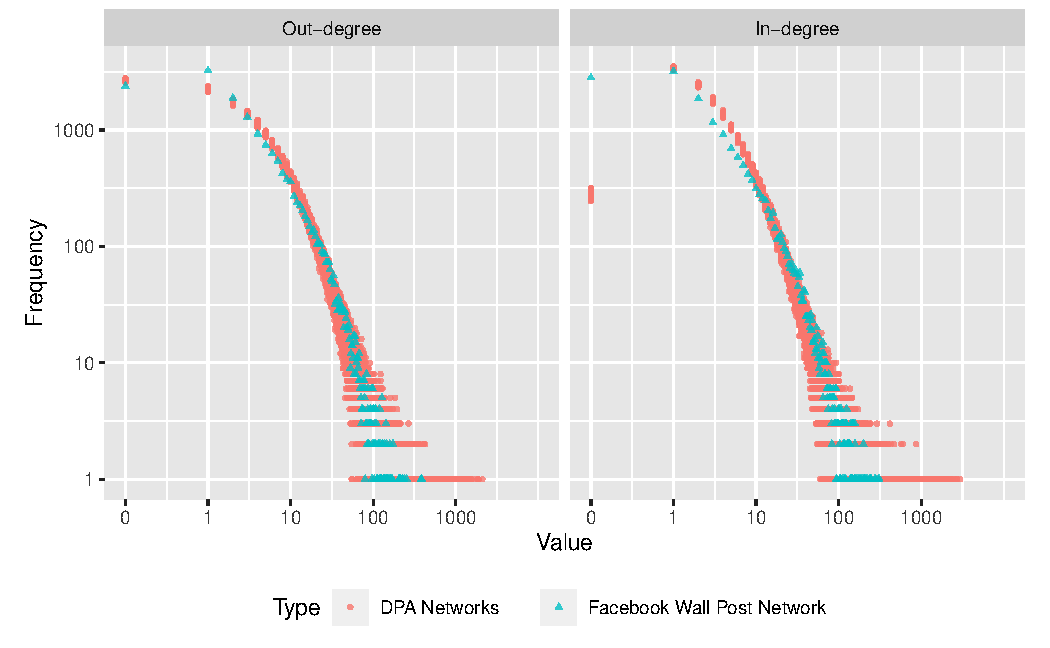
\includegraphics[width=0.8\linewidth]{facebook_degree-compressed.pdf}
\end{figure}
	
\end{frame}

%------------------------------------------------

\begin{frame}{Facebook wall post network}

This figure shows the average trace plots of the assortativity coefficients
based on the $100$ simulated DPA networks, where the assortativity values of
each kind are updated every $10^3$ rewiring steps. 

% After rewiring, all of the assortativity coefficients are 
% close to their counterparts observed from the selected sub-network, thus
% filling up the discrepancy in the simple DPA model.

\begin{figure}
	\centering
	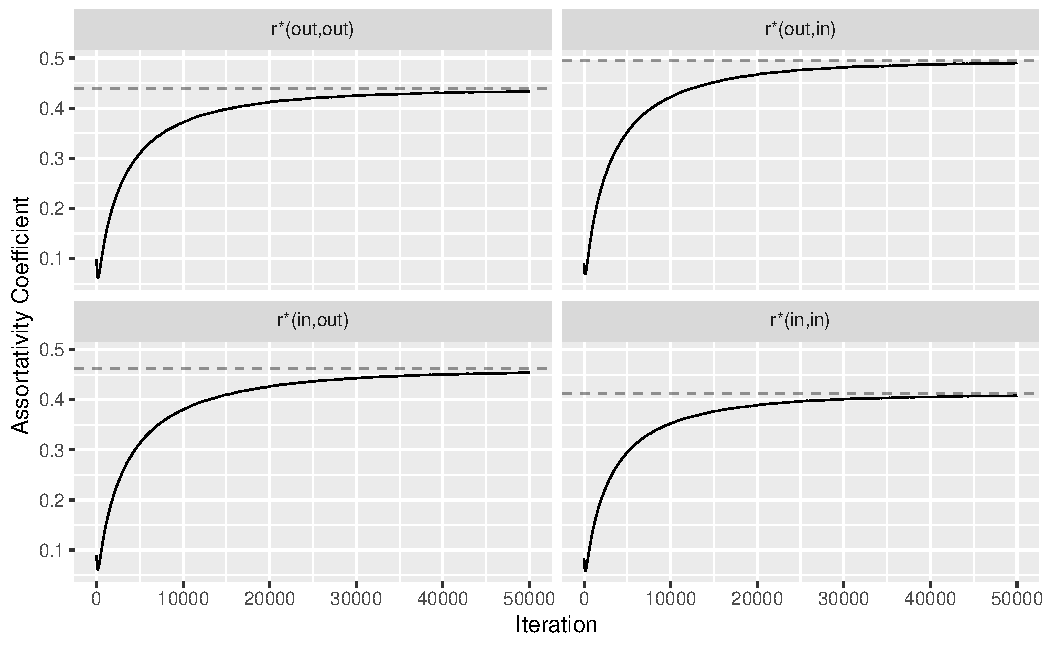
\includegraphics[width=0.8\linewidth]{facebook_resized_archive.pdf}
\end{figure}
	
\end{frame}

%------------------------------------------------

\appendix

\begin{frame}[plain]{Discussion}

\begin{itemize}
	\item The proposed DiDPR algorithm
	corrects assortativity coefficients while preserving node out- and in-degree distributions, but does not account for other network characteristics, such as
	community structure, clustering coefficient, or centrality measures.
	\item The rewiring algorithm may create self-loops
	and multiple edges.
	\item The algorithm does not consider weighted networks.
\end{itemize}
	
\end{frame}

%------------------------------------------------

\begin{frame}[plain]{References}
	\fontsize{7}{8}\selectfont
	\nocite{Wang2022generating}
	\nocite{Rpkg:wdnet}
	\bibliographystyle{chicago}
	\bibliography{refs}
\end{frame}

%------------------------------------------------

\end{document}
